\section*{Введение}
\addcontentsline{toc}{section}{Введение}

Астрофизический $r$-процесс, или процесс быстрого нейтронного захвата, является механизмом нуклеосинтеза, в ходе которого исходное ядро поглощает большое число нейтронов и, оказавшись в области нейтронного избытка, испытывает слабые распады. В результате масса ядра увеличивается за счет поглощенных нейтронов, а $\beta^-$-распады приводят к образованию химического элемента с большим зарядовым числом. В $r$-процессе скорости нейтронного захвата на порядки превышают скорости $\beta^-$-распадов, что обеспечивает стремительный набор массы и значительное смещение в область нейтронного избытка. Для достижения необходимой интенсивности поглощения нейтронов требуется высокая плотность их потока, около 150 нейтронов на одно зародышевое ядро, и температуры вещества свыше 1~ГК. Такие экстремальные условия могут реализовавываться при катастрофических явлениях: взрывах сверхновых, слияниях двух нейтронных звезд, слияниях нейтронной звезды и черной дыры. 

По современным представлениям, именно $r$-процесс обеспечивает возникновение основной массы ядер химических элементов тяжелее железа во Вселенной. Синтез более легких ядер обеспечивается термоядерным горением звездного вещества, но, как известно, им невозможно объяснить возникновение химических элементов за так называемым <<железным пиком>>, максимумом зависимости удельной энергии связи от массового числа. Процесс медленного нейтронного захвата, или $s$-процесс, отличающийся от $r$-процесса значительно меньшей интенсивностью поглощения нейтронов и, соответственно, характерными временами порядка сотен лет, требует не столь исключительных астрофизических условий и обеспечивает образование ядер вблизи долины стабильности вплоть до свинца и висмута. Однако $s$-процессом нельзя объяснить существование более тяжелых ядер, а также нейтроноизбыточных изотопов, слишком удаленных от долины стабильности. Некоторое количество обойденных протоноизбыточных изотопов возникает в $p$-процессе, механизме взровного нуклеосинтеза, представляющем собой последовательности фотоядерных реакций и поглощений заряженных частиц. Однако выходы $p$-процесса малы по сравнению с $s$- и $r$-процессами. Кроме того, для синтеза $p$-изотопов требуется наличие достаточно тяжелых стабильных ядер, достаточное число которых может образоваться только в результате процессов нейтронного захвата. 

На рис.~\ref{fig:lodders_vs_ame} показано массовое распределение ядер в Солнечной системе, построенное по данным~\cite{lodders2003}. Виден избыток легчайших изотопов с $A \leq 4$, родившихся в первичном нуклеосинтезе, за которым следует минимум, соответствующий изотопам $Li$, $Be$ и $B$. С массового числа 12 начинается область ядер, рождающихся в основном в процессе термоядерного горения звездного вещества, включающем, в частности, pp- и CNO-циклы. Видно, что начиная с массовых чисел $54 - 58$, соответствующих <<железному пику>>, начинается резкое снижение концентраций изотопов. В области более тяжелых ядер нуклеосинтез целиком обеспечивается $s$- и $r$-процессами. На рис.~\ref{fig:lodders_vs_ame} отмечены характерные пики, соответствующие магическим числам нейтронов 50, 82 и 126, что является указанием на высокий вклад процессов нейтронного захвата в нуклеисинтез. Более узкие пики образуются благодаря $s$-процессу, который протекает вблизи долины стабильности, в то время как $r$-процесс рождает сверх-нейтроноизбыточные ядра, которые могут терять массу вследствие слабых распадов с вылетом нескольких нейтронов. Это приводит к уширению смещению пиков $r$-процесса влево.

\begin{figure}
  \centering
  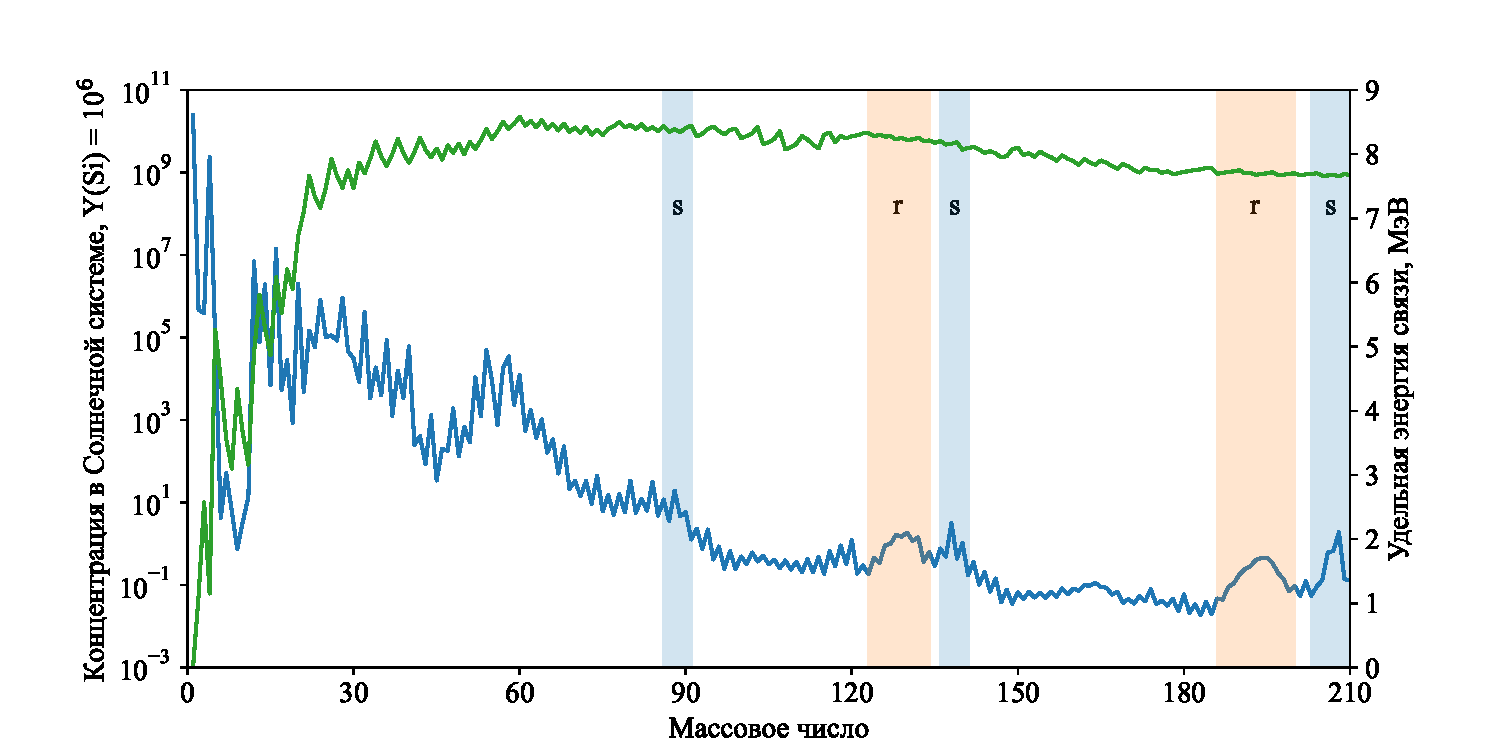
\includegraphics[width=0.8\textwidth]{pics/lodders_vs_ame.pdf}
  \caption{Массовое распределение ядер в Солнечной системе по данным~\cite{lodders2003}, масса изотопов Si принята равной $10^6$. Оранжевым отмечены пики $r$-процесса, синим --- пики $s$-процесса (согласно~\cite{cowan2021}).}
  \label{fig:lodders_vs_ame}
\end{figure}

Основным методом исследования $r$-процесса и эволюции астрофизических ядерных систем в целом является математическое моделирование. Для получения надежных результатов симуляции необходимо достоверно знать ряд входных параметров, таких как состав звездного вещества, его температуры и плотности, а также сечения ядерных реакций, протекающих в звездах. На данный момент эти величины известны в основном из теоретических моделей, астрофизических и ядерных, что вызывает существенные неопределенности входных данных.


